\documentclass[border=10pt]{standalone}

\usepackage{tikz}
\usepackage{tikzsymbols}
\usetikzlibrary{calc,patterns,shapes.geometric}

\def\centerarc[#1](#2)(#3:#4:#5){\draw[#1] ($(#2)+({#5*cos(#3)},{#5*sin(#3)})$) arc (#3:#4:#5);}

\begin{document}
	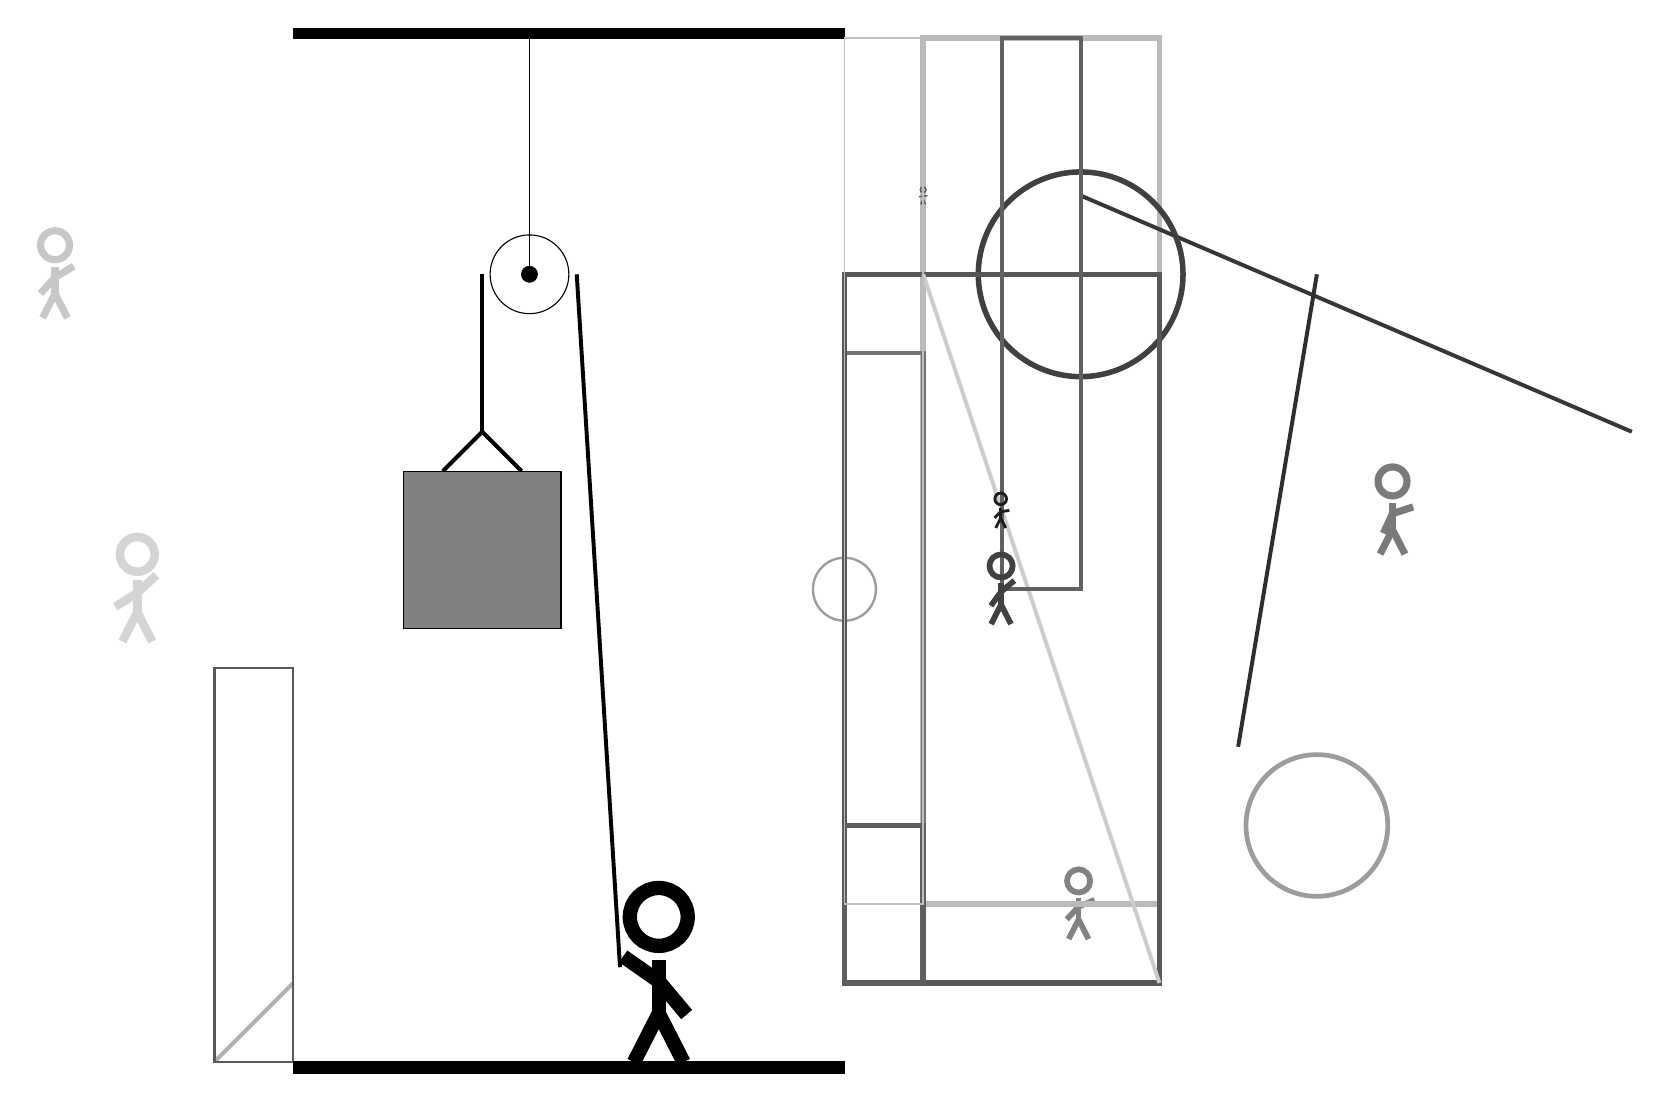
\begin{tikzpicture}
		%%%%% START %%%%%
		
		\draw[fill=black] (-2, 10) rectangle (5, 10.125);
		
		\draw (1, 7) circle (0.5);
		\draw[fill=black] (1, 7) circle (0.1);
		\draw (1, 10) -- (1, 7);
		
		\draw[line width=0.5mm] (-0.1, 4.5) -- (0.4, 5.0) -- (0.9, 4.5);
		\draw[fill=black!50] (-0.6, 4.5) rectangle (1.4, 2.5);
		
		\node[line width=0.5mm, color=black!49] at (8, -1) {\Strichmaxerl[4][47][23]};
		
		\draw[line width=0.7mm, color=black!27] (6, -1) rectangle (9, 10);
		\draw [line width=0.3mm, color=black!39](5, 3) circle (0.4);
		\draw[line width=0.5mm, color=black!30](-2, -2) -- (-3, -3);
		\draw[line width=0.5mm, color=black!79](8, 8) -- (15, 5);
		
		\node[line width=0.7mm, color=black!22] at (-5, 7) {\Strichmaxerl[5][48][31]};
		\draw [line width=0.6mm, color=black!39](11, 0) circle (0.9);
		
		\draw[line width=0.6mm, color=black!55] (6, 6) rectangle (5, 0);
		\draw [line width=0.7mm, color=black!75](8, 7) circle (1.3);
		\draw[line width=0.7mm, color=black!66] (5, 7) rectangle (9, -2);
		\draw[line width=0.5mm, color=black!20](6, 7) -- (9, -2);
		\draw[line width=0.5mm, color=black!62] (7, 3) rectangle (8, 10);
		\node[line width=0.7mm, color=black!52] at (12, 4) {\Strichmaxerl[5][65][18]};
		
		\node[line width=0.3mm, color=black!17] at (-4, 3) {\Strichmaxerl[6][32][43]};
		\draw[line width=0.5mm, color=black!82](10, 1) -- (11, 7);
		\draw [line width=0.3mm, color=black!36](-4, 6) circle (0.0);
		\node[line width=0.6mm, color=black!64] at (6, 8) {\Strichmaxerl[1][8][7]};
		\draw[line width=0.7mm, color=black!63] (5, -2) rectangle (6, 0);
		\node[line width=0.7mm, color=black!89] at (7, 4) {\Strichmaxerl[2][45][9]};
		\draw[line width=0.3mm, color=black!65] (-3, 2) rectangle (-2, -3);
		\draw[line width=0.2mm, color=black!25] (5, 10) rectangle (6, -1);
		
		\node[line width=0.3mm, color=black!75] at (7, 3) {\Strichmaxerl[4][54][40]};
		
		
		\draw[line width=0.5mm] (0.4, 7) -- (0.4, 5.0);
		\centerarc[line width=0.5mm](1, 7)(0:180:0.6);
		\draw[line width=0.5mm](1.6, 7) -- (2.15, -1.8);
		
		\node at (2.6, -1.9) {\Strichmaxerl[10][-35][-50]};
		
		\draw[fill=black] (-2, -3) rectangle (5, -3.15);
		
		%%%%% END %%%%%
	\end{tikzpicture}
\end{document}